% lualatex statestikz-3.tex
% pdf2svg statestikz-3.pdf statestikz-3.svg

\documentclass[border=2bp, tikz]{standalone}
\usepackage{tikz}

\usetikzlibrary{calc,trees,matrix,positioning,chains,fit,intersections}
\usetikzlibrary{arrows,shapes.arrows,shapes.geometric,shapes.multipart,shapes.symbols}
\tikzset{
   state/.style={ rectangle, draw=black, thick, minimum height=1.66em, text centered, rounded corners=3pt},
   partial state/.style={trapezium, draw=black, thick, minimum height=1.66em, text centered, rounded corners=3pt},
   error state/.style={ rectangle, double, draw=black, semithick, minimum height=1.66em, text centered, rounded corners=3pt},
   off state/.style={ circle, double, draw=black, semithick, minimum height=1.66em, text centered, rounded corners=3pt},
   branch/.style={ fill, shape=circle, minimum size=3pt, inner sep=0pt},
   cross line/.style={preaction={draw=white, -, shorten >=3pt, shorten <=3pt, line width=2pt}},
   >=latex
}
\usepackage{fontspec}
\setmainfont[UprightFont={Petrona-Light.ttf},
             BoldFont={Petrona-Medium.ttf},
             ItalicFont={Petrona-LightItalic.ttf},
             BoldItalicFont={Petrona-MediumItalic.ttf},
            ]{Petrona-Light.ttf}

\begin{document}
\begingroup
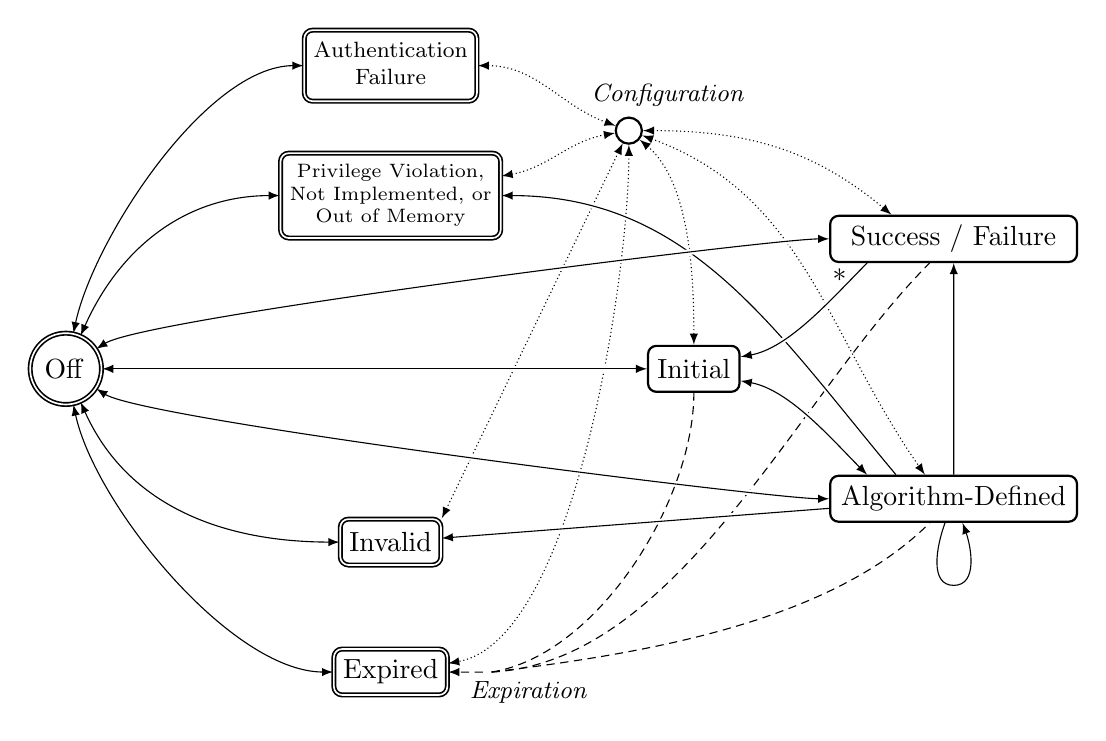
\begin{tikzpicture}[scale=1.1]

  \node[off state]   at (-1.75,0)    (off)            {Off\,};

  \node[error state] at (2,-2)    (invalid)        {Invalid};
  \node[error state] at (2,2)     (various errors) {\scriptsize\begin{tabular}{@{}c@{}}Privilege Violation,\\Not Implemented, or\\Out of Memory\end{tabular}};
  \node[error state] at (2,3.5)   (authfail)       {\footnotesize\begin{tabular}{@{}c@{}}Authentication\\Failure\end{tabular}};
  \node[error state] at (2,-3.5)  (expired)        {Expired};

  \node[circle,thick,draw=black] at (4.75,2.75) (configuration hub) {};
  \node[coordinate] at ($(expired.east)+(0.5,0)$) (before expired) {};

  \node[state, thick] at (5.5,0)    (initial)           {Initial};
  \node[state, thick, text width=2.9cm] at (8.5,-1.5) (algorithm defined) {Algorithm-Defined};
  \node[state, thick, text width=2.9cm] at (8.5,1.5)  (success failure)   {Success / Failure};

  %%%%%%%%%%%

  \node[above=0mm  of configuration hub,xshift=5mm] (ignore) {\small\textit{Configuration}};
  \node[below right=0mm and -4mm of before expired] (ignore) {\small\textit{Expiration}};

  %%%%%%%%%%%

  \draw[-,densely dashed]   (before expired) to[out=9,in=270,looseness=0.8] (initial);
  \draw[-,densely dashed]   (before expired) to[out=7,in=225,looseness=0.8] (algorithm defined);
  \draw[-,densely dashed]   (before expired) to[out=3,in=225,looseness=0.8] (success failure);
  \draw[->,densely dashed]  ($(before expired)+(-0.1,0)$) -- (expired);

  \draw[<->,densely dotted] (configuration hub) to[out=-40,in=90,looseness=0.8] (initial);
  \draw[<->,densely dotted] (configuration hub) to[out=-20,in=125] ($(algorithm defined.north)+(-0.333,0)$);
  \draw[<->,densely dotted] (configuration hub) to[out=0,in=140] ($(success failure.north)!0.5!(success failure.north west)$);
  \draw[<->,densely dotted] (configuration hub) to[out=160,in=0] (authfail);
  \draw[<->,densely dotted] (configuration hub) to[out=190,in=10] (various errors);
  \draw[<->,densely dotted] (configuration hub) -- (invalid.north east);
  \draw[<->,densely dotted] (configuration hub) to[out=270,in=10,looseness=0.6] ($(expired.east)+(0,0.1)$);

  \draw[<->] (off) to[out=-66,in=180] (invalid);
  \draw[<->] (off) to[out=78,in=180,looseness=0.7] (authfail);
  \draw[<->] (off) to[out=66,in=180] (various errors);
  \draw[<->] (off) to[out=-78,in=180,looseness=0.7] (expired);

  \draw[->] (algorithm defined) to[out=250,in=180] ($(algorithm defined)+(0,-1)$) to[out=0,in=290] (algorithm defined);
  \draw[->, cross line] (algorithm defined) -- (invalid);
  \draw[->,cross line] ($(algorithm defined.north)+(-0.667,0)$) to[out=130,in=0] (various errors);

  \draw[<->,cross line] (off) -- (initial);
  \draw[<->,cross line] (off) to[out=-33,in=180,looseness=0.2] (algorithm defined);
  \draw[<->,cross line] (off) to[out=33,in=180,looseness=0.2] (success failure);

  \draw[->,cross line]  ($(success failure.south)+(-1,0)$)   to[out=225,in=10,looseness=0.8] node[near start, above, yshift=-3pt] () {*} ($(initial.east)!0.5!(initial.north east)$);
  \draw[<->,cross line] ($(algorithm defined.north)+(-1,0)$) to[out=135,in=-10,looseness=0.8] ($(initial.east)!0.5!(initial.south east)$);
  \draw[->,cross line] (algorithm defined) -- (success failure);

\end{tikzpicture}
\endgroup
\end{document}
